\section{Initial Prototype}
As previously stated, living with a mental illness can be isolating and the stigma around mental health issues makes people hesitant to seek professional help. The primary purpose of this thesis is to create a functional prototype capable of connecting people with mental health specialists anonymously, while still maintaining client-therapist empathy.

A working prototype was developed using Unreal Engine Blueprints (a node-based interface to create gameplay elements), the UE4, Metahumans, and Live Link connected to an iPhone's camera. In the prototype, patients can communicate with mental health specialists via video conferencing anonymously, as patient's smartphone functions as a virtual camera that allows the mental health practitioner to see the patient's facial expressions in real-time via a virtual avatar. 

Using an Apple device with the TrueDepth sensor and the Live Link Face app, one can capture numerous facial tracking points by creating a depth map of ones’ face while projecting and analyzing over 30,000 invisible dots, as well as capturing an infrared face image. The data collected by the Apple device and app is delivered to the UE4 environment via a directed internet connection maintained between the user's iPhone/iPad and the Unreal Engine. When data is received by Unreal Engine 4, it is evaluated and turned into virtual avatar movements via Live Link Plugin, as shown in Figure 1 and Figure 2.

\begin{figure}[h!]
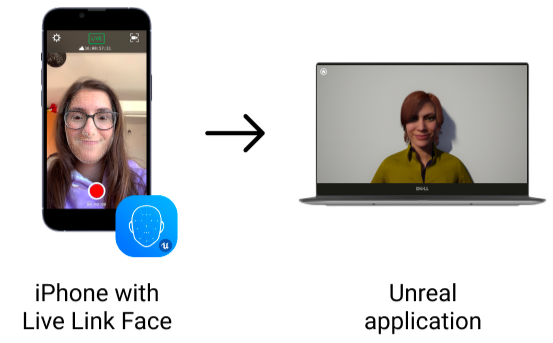
\includegraphics[width=0.45\textwidth]{figures/howItWorks.png}
\centering
\caption{How the facial expressions are captured and represented}
\end{figure}

\begin{figure}[h!]
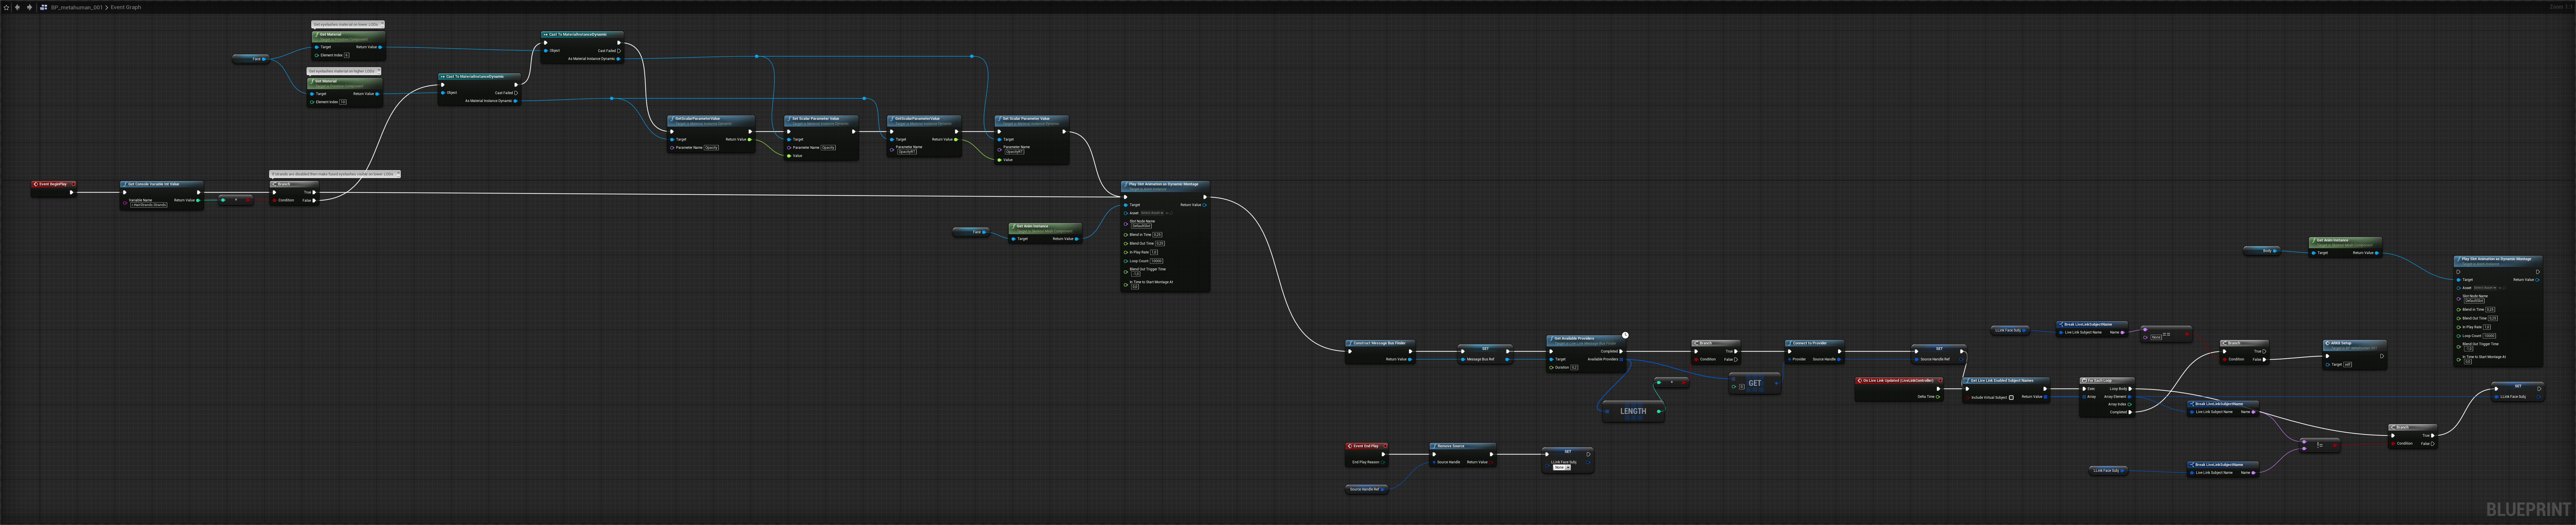
\includegraphics[width=0.49\textwidth]{figures/hereItBegins.png}
\centering
\caption{Blueprints responsible for the connection and stream of data}
\end{figure}

The goal of the Live Link Plugin \cite{EPI22} is to provide a unified interface for streaming and consuming animation data into Unreal Engine 4 from one or more external sources, such as Display Data Channel (DDC) tools or Mocap Servers. It's built to be extensible via Unreal Plugins, allowing third parties to create new features without having to make and maintain Engine changes. Live Link can also be used by Motion Capture Systems to stream data into the Engine that can be previewed in real time.

To provide users with options, and thus reach a wider audience, four metahumans (two males and two females, of different ethnicities) were exported from the Metahuman Creator \cite{EPI21}, and the Quixel Bridge application into UE4, where, in order to make the interaction with the prototype easier, a minimalist user interface (Figure 4) was created that allows users to choose their preferred avatar. 

Although custom metahumans were not employed in this version of the prototype, due to performance and optimization concerns, the chosen metahumans (Figure 3) were pre-made by Epic Games and available on Quixel Bridge. These concerns were alleviated by using these four metahumans because Epic Games pre-defines export settings and assets compatible with many devices.

\begin{figure}[h!]
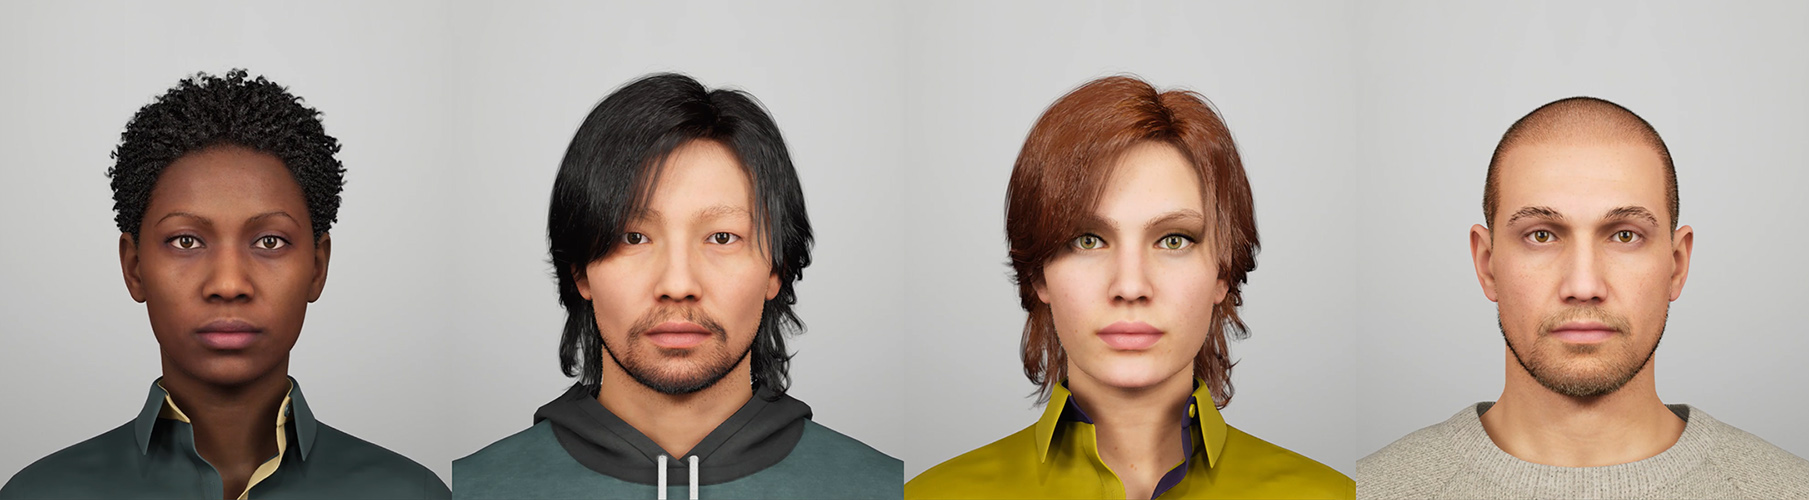
\includegraphics[width=0.49\textwidth]{figures/4metahumans.jpg}
\centering
\caption{The current metahumans used on the prototype}
\end{figure}


\begin{figure}[h!]
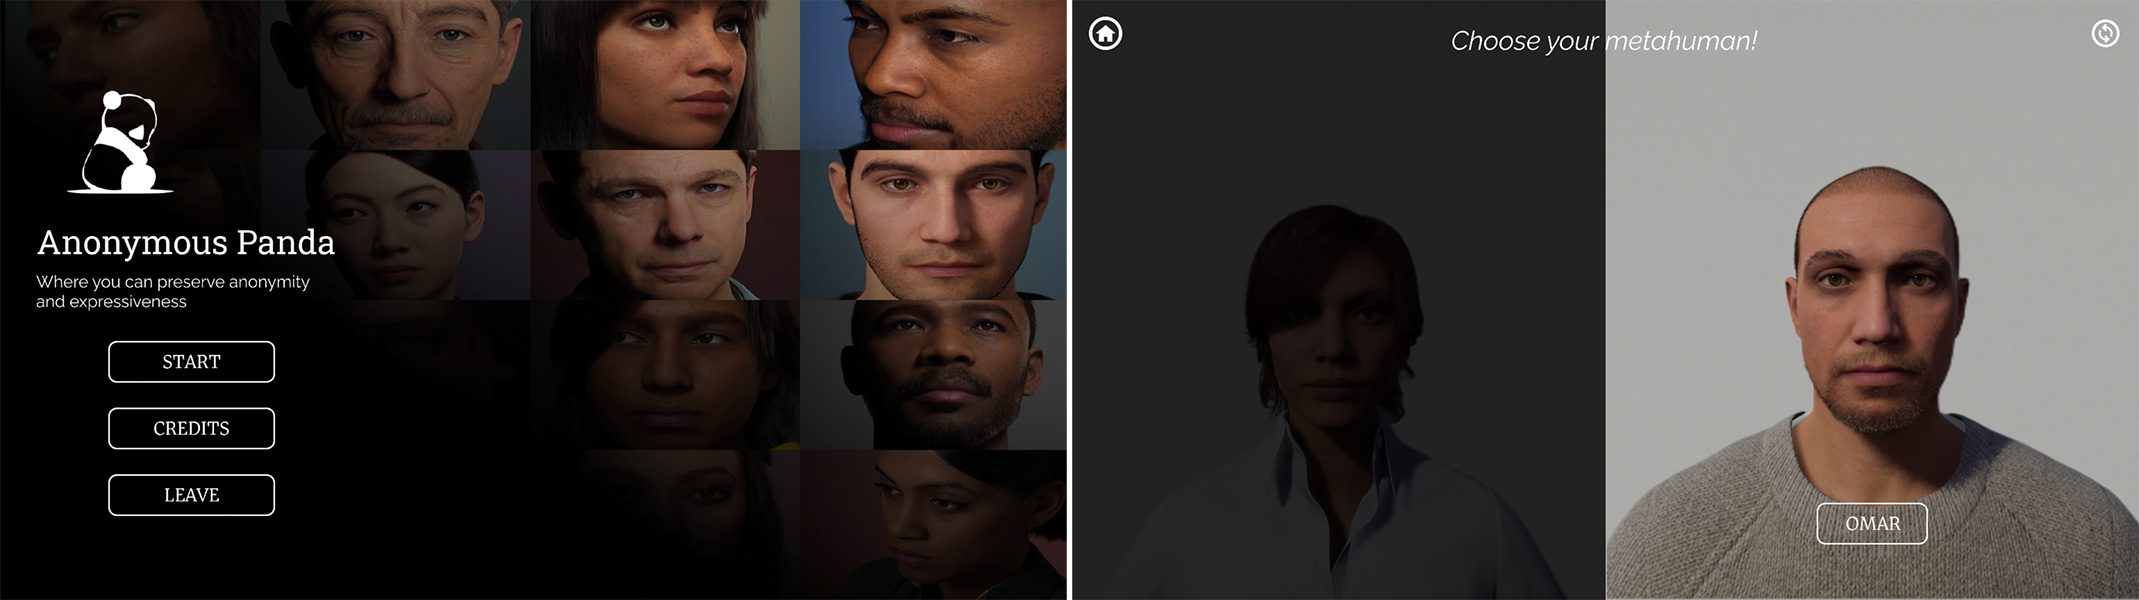
\includegraphics[width=0.49\textwidth]{figures/ui-app.jpg}
\centering
\caption{Screenshots of the Anonymous Panda application}
\end{figure}

The human face is the primary means of non-verbal communication \cite{MALO20, KUJ03, SAU19}, used to communicate one's emotions and mood, and to provide visual cues of a person's physical state. Facial expressions are easily distinguished across cultures and automatically perceived so that we can immediately evaluate someone's emotional state. As Figure 5 makes visible, the facial expression of the virtual avatars are perceptible in the current version of the prototype. 

\begin{figure}[h!]
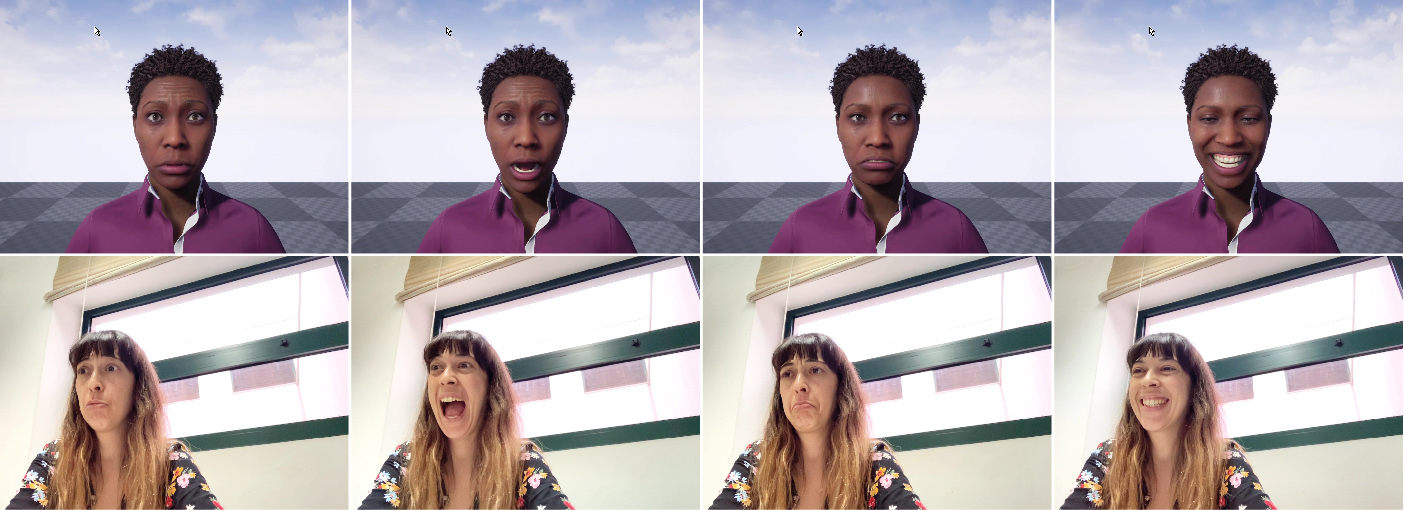
\includegraphics[width=0.49\textwidth]{figures/expressionTest.jpg}
\centering
\caption{Examples of facial expressions and their virtual avatar depiction}
\end{figure}

However, upon a closer look, even though the avatar could accurately represent the user's facial expressions using the default functions of the live link plugin, a minor flaw in terms of lip positioning was found, particularly when the mouth should be closed or when the user was trying to express a negative emotion (e.g., sadness). To solve this issue, the upper lip values were slightly adjusted (Figure 6) before being reconverted to metahuman animation.

\begin{figure}[h!]
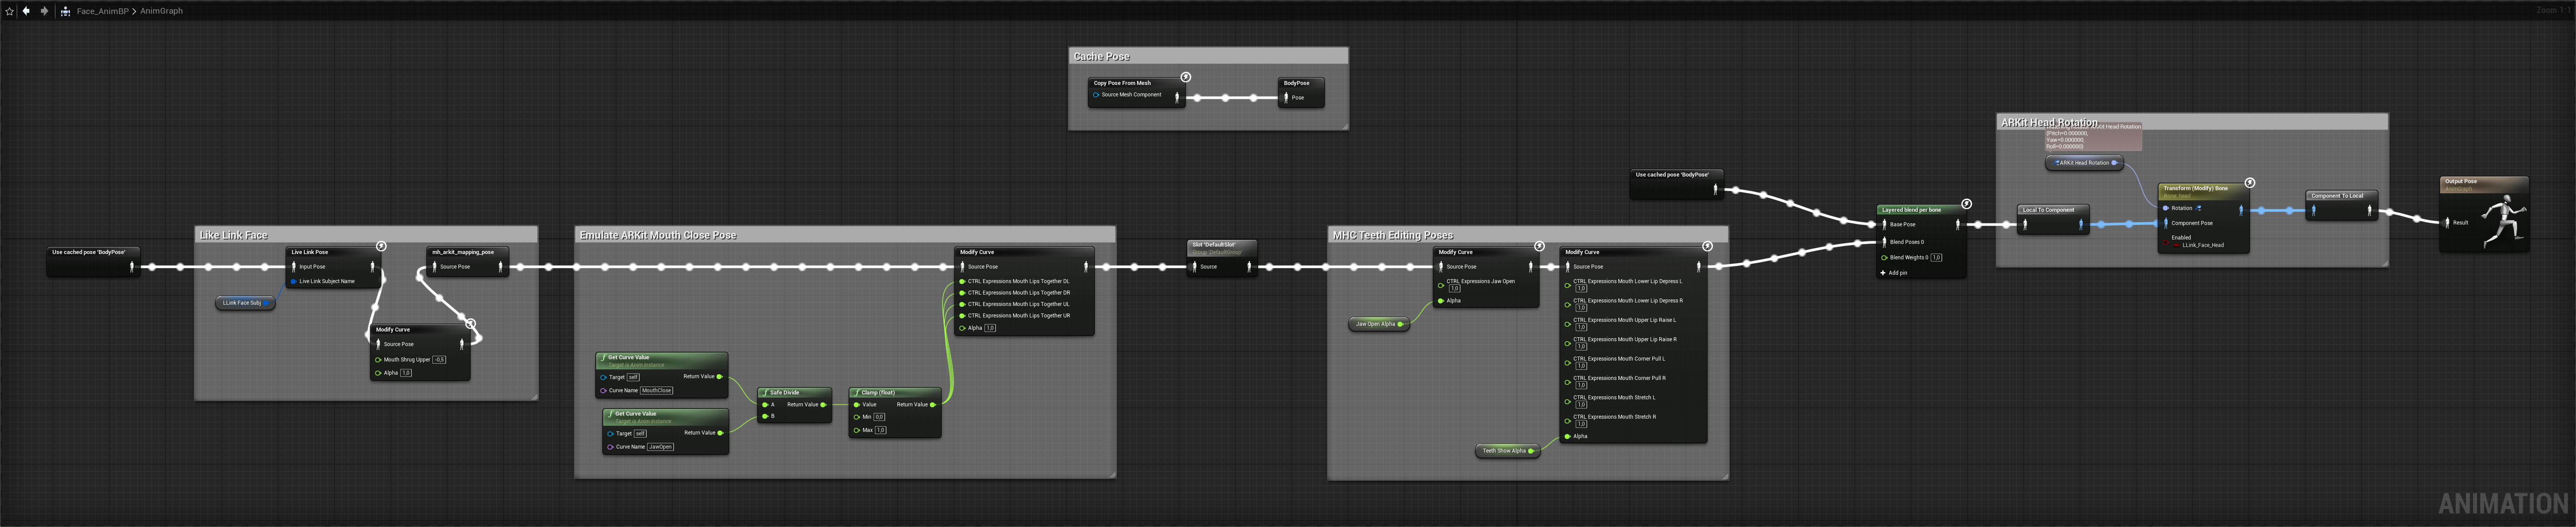
\includegraphics[width=0.49\textwidth]{figures/facialConfig.png}
\centering
\caption{Blueprints responsible for the conversion of data to animation of metahuman}
\end{figure}

Although one of the foundations of this thesis is doctor-patient communication, the current prototype uses the UE4 application to emulate a webcam; meaning the user has to share their screen via a video conferencing tool (Figure 7). Even though this causes a slight delay, it can be used in a video conference.

\begin{figure}[h!]
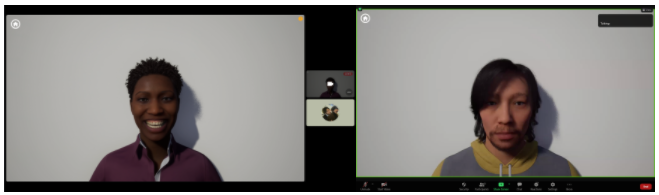
\includegraphics[width=0.49\textwidth]{figures/zoomAndDiscord.PNG}
\centering
\caption{The prototype in use on a call via Discord and Zoom}
\end{figure}

\subsection{Limitations}
One of the thesis's challenges is to use customized models because these models demand a lot of optimization. After all, they are resource-intensive, limiting the patient's expressions from being viewed clearly and fluidly. Because this is a resource-intensive application, another difficulty is how people will utilize it. As a result, one of the problems is figuring out how to develop this program to reach everyone who needs it. Finally, improving the patients' expressions through hand tracking is another challenge. We can learn new ways for people to express themselves and improve mental health professionals' understanding by using hand tracking.

\subsection{Future Work}
\subsubsection{Custom Metahumans}
The creation and use of custom metahumans has already improved thanks to recent contributions from Epic Games. However, because many assets are still in development, the creation and use of metahumans is still limited; however, if these assets are excluded, it should be possible to use metahumans other than those pre-defined by Epic Games.

\subsubsection{Hand Tracking}
While there are a variety of ways to perform hand tracking, such as with virtual reality devices or gloves, we believe that the leap motion controller is the best option for this project because it is a practical and small device that does not interfere with the face recognition part.

The Leap Motion Controller (Figure 8) is a device that connects to a PC or a Mac and allows users to manipulate digital objects using hand motions. It adds a new way to interact with the digital world when combined with other hardware. Programs that interpret gesture-based computing allow users to play games, design, and learn in a hands-on manner. This device maps and tracks the human hand using an infrared scanner and sensor. This data is used to create a digital version of the hand that can manipulate digital objects in real time.

\begin{figure}[h!]
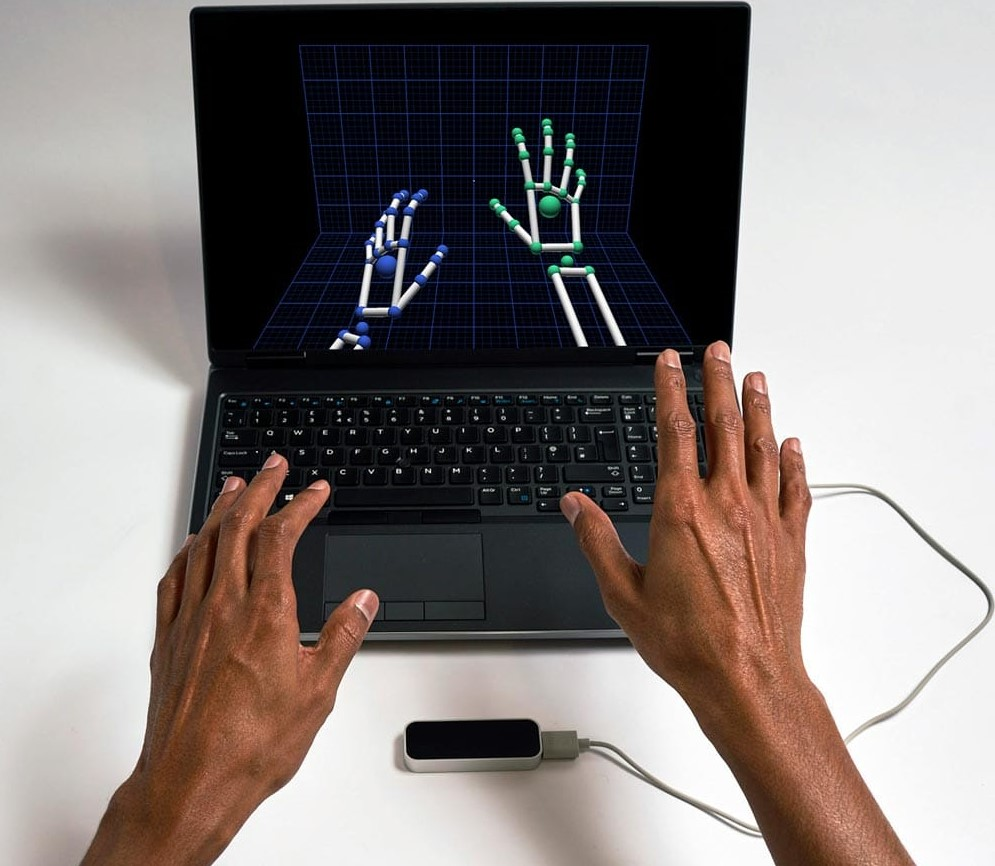
\includegraphics[width=0.2\textwidth]{figures/leapMotion.jpg}
\centering
\caption{Example of the leap motion tracking}
\end{figure}

The Ultraleap Unreal Plugin \cite{ULT} allows developers to use the data generated by integrating Ultraleap's hand tracking data in their Unreal projects. It was created with the goal of designing and implementing hand tracking in Extended Reality (XR) projects. Despite the difficulty, it may be possible to adapt the use of this plugin to this work with the right changes.

Meanwhile, by introducing this device, we are introducing a new limitation. The fact that, despite being more affordable than an Apple device with the TrueDepth sensor, this device is more difficult to obtain because it is sold in fewer stores.
